\documentclass[12pt]{article}
%\usepackage{times}
%\usepackage[T1]{fontenc}
%\usepackage[latin1]{inputenc}
\usepackage{geometry}
%\usepackage[dvips]{color,graphics}
\usepackage{longtable}
\usepackage{hyperref}
\usepackage[pdftex]{graphicx}
\usepackage[absolute,overlay]{textpos}
\usepackage{graphicx}
\usepackage{relsize}
\usepackage{epstopdf}
\usepackage{setspace}
\usepackage{epsf}
\usepackage{amsmath}
\usepackage{amssymb}
\usepackage{epstopdf}
\usepackage{setspace} 
\usepackage{parallel}
\usepackage{multirow}
\DeclareGraphicsRule{.tif}{png}{.png}{`convert #1 `dirname #1`/`basename #1 .tif`.png}
\usepackage{rotating}

\setlength{\TPHorizModule}{1mm}
\setlength{\TPVertModule}{1mm}
%
\textwidth  6.5in
\textheight 9.0in
\topmargin 0.0 in
\headheight 0.0in
\headsep 0.0in
\oddsidemargin 0in
\evensidemargin 0in
\parsep 0 in
%\parindent 0in
\pagenumbering{arabic}
%
\setcounter{secnumdepth}{5}
\setcounter{tocdepth}{5}
%\usepackage{geometry}
%\usepackage{fancyhdr}
%left=1.5in,right=1in,top=1in,bottom=1in
%\geometry{verbose,letterpaper,tmargin=0.8in,bmargin=0.7in,lmargin=0.5in,rmargin=0.5in}
\geometry{verbose,a4paper,tmargin=1in,bmargin=1in,lmargin=1.3in,rmargin=1in}
\pagestyle{plain}
\setcounter{secnumdepth}{3}
\setcounter{tocdepth}{3}


 
\makeatletter
 
 
%%%%%%%%%%%%%%%%%%%%%%%%%%%%%% LyX specific LaTeX commands.
\providecommand{\LyX}{L\kern-.1667em\lower.25em\hbox{Y}\kern-.125emX\@}
%% This length is the backup for minipages of the \parindent
\newlength{\LyXMinipageIndent}
\setlength{\LyXMinipageIndent}{\parindent}
%% Special footnote code from the package 'stblftnt.sty'
%% Author: Robin Fairbairns -- Last revised Dec 13 1996
\let\SF@@footnote\footnote
\def\footnote{\ifx\protect\@typeset@protect
    \expandafter\SF@@footnote
  \else
    \expandafter\SF@gobble@opt
  \fi
}
\expandafter\def\csname SF@gobble@opt \endcsname{\@ifnextchar[%]
  \SF@gobble@twobracket
  \@gobble
}
\edef\SF@gobble@opt{\noexpand\protect
  \expandafter\noexpand\csname SF@gobble@opt \endcsname}
\def\SF@gobble@twobracket[#1]#2{}
 
\makeatother


\def\lambdabar{\protect\@lambdabar}
\def\@lambdabar{%
\relax
\bgroup
\def\@tempa{\hbox{\raise.73\ht0
\hbox to0pt{\kern.25\wd0\vrule width.5\wd0
height.1pt depth.1pt\hss}\box0}}%
\mathchoice{\setbox0\hbox{$\displaystyle\lambda$}\@tempa}%
{\setbox0\hbox{$\textstyle\lambda$}\@tempa}%
{\setbox0\hbox{$\scriptstyle\lambda$}\@tempa}%
{\setbox0\hbox{$\scriptscriptstyle\lambda$}\@tempa}%
\egroup
}
%\fancyhead[]{}
%\fancyhead[]{}
\begin{document}
%\frontmatter
%\pagestyle{plain}
%\thispagestyle{empty}
\title{Central Neutron Detector Operations Manual}

\vskip 0.5cm

\author{S. Niccolai, IPN Orsay\\[0.2ex]
{\it cnd\_manual.tex -- v1.2}}

\date \today
\maketitle
%\input{title_ops}
\begin{abstract}This document describes the Central Neutron Detector (CND) of CLAS12, and the procedures to operate it and to monitor its correct functioning. 
\end{abstract}
\newpage
\thispagestyle{empty}

\pagenumbering{roman}
 
\setcounter{page}{1}
 
\tableofcontents{}
 
%\listoftables{}
 
%\listoffigures{}
 
\newpage 
\pagenumbering{arabic}
%\fancyhead[]{}
%\pagestyle{fancy}
%\chead[]{\let\uppercase\relax\leftmark}
\setcounter{page}{1}
\section{Description of the detector}\label{cnd-section}
The Central Neutron Detector (CND) is the outermost detector of the Central-Detector part of CLAS12. It contains the CTOF and the Central Tracker. 

The CND is a barrel of plastic scintillator bars of trapezoidal shape, all with their long sides parallel to the beam direction (Fig.~\ref{geom_scint}). 

\begin{figure}
\begin{center}
\centering
\resizebox{0.58\textwidth}{!}{\includegraphics{Geometriescintillateurs.pdf}}
\caption {Geometry of the scintillator barrel for the Central Neutron Detector. It consists of 3 radial layers each made of 48 trapezoidal scintillator paddles.}
\label{geom_scint}
\end{center}
\end{figure}

The light emitted by the scintillators of the CND is read only at the backward end of each bar, with an Hamamatsu R10533 photomultiplier placed in the low-field region of the solenoid, and connected to the bar by a $\sim 1.5$-m-long bent light guide; the front end of the bar is connected via a ``u-turn'' light guide to the neighboring paddle. This way, the light emitted at the front end of one scintillator is fed through its neighboring paddle and read by the PMT connected to its end (Fig.~\ref{cnd_nice}). Each PMT is encased in a cylindrical shielding made up by a 1-mm-thick layer of mu-metal and a 5-mm-thick layer of mild steel. 

\begin{figure}
\begin{center}
\centering
\resizebox{1.2\textwidth}{!}{\includegraphics{CND_bello.pdf}}
\vspace{-2.5cm}
\caption {Design of the Central Neutron Detector, inserted in the CLAS12 solenoid.}
\label{cnd_nice}
\end{center}
\end{figure}

The detector is to composed by 48 azimuthal segments and 3 layers in the radial direction, for a total of 144 scintillator bars, 144 PMTs, 72 u-turn light guides, 144 bent light guides (Fig.~\ref{cnd_nice}). 

In order to operate the PMTs, high voltages (typically in the range of 1500 V) are provided to them by multi-channel CAEN SY527 power supplies (Fig.~\ref{hv_ps_figure}, left). The HV boards adopted for the CND are CAEN A734N (16 channels, 3 kV max voltage, 3 mA max current) (Fig.~\ref{hv_ps_figure}, right). 
\begin{figure}
\begin{center}
\resizebox{0.55\textwidth}{!}{\includegraphics{caen_front.pdf}}
\resizebox{0.31\textwidth}{!}{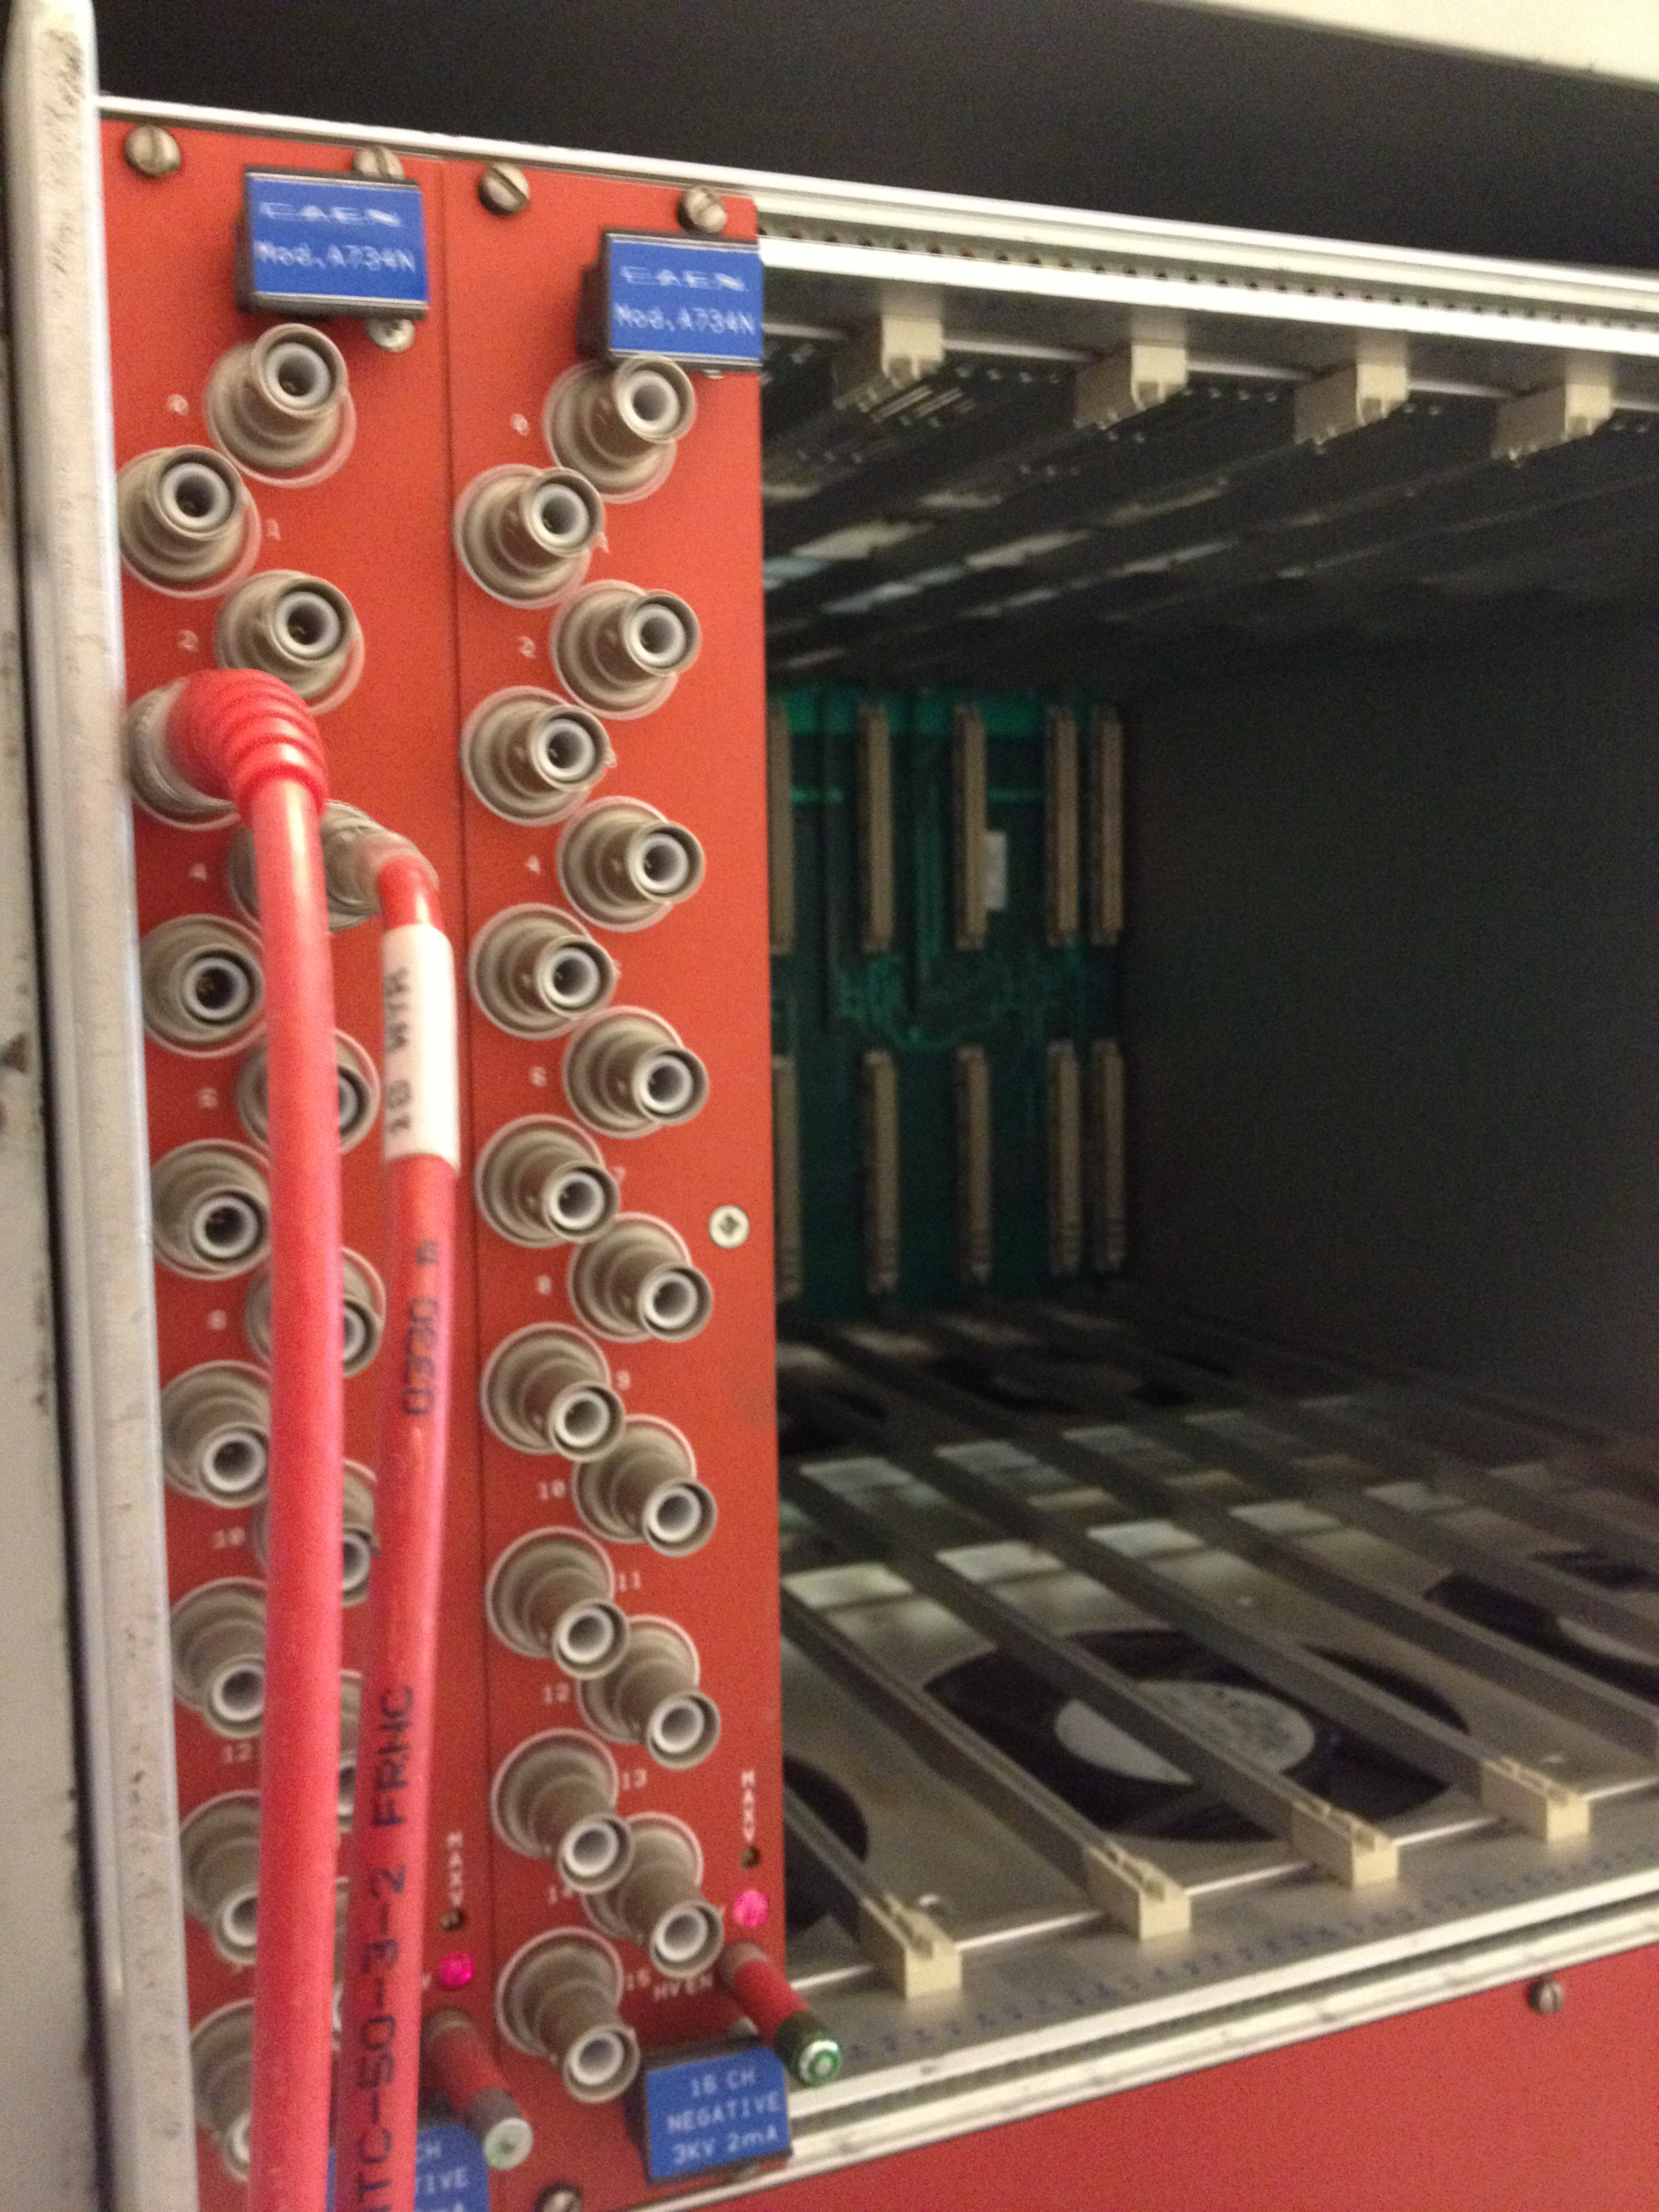
\includegraphics{IMG_4869.png}}
\caption {Left: Front panel of the HV power supply for the PMTs of the CND. Right: HV boards.}
\label{hv_ps_figure}
\end{center}
\end{figure}
\section{Read-out electronics}
Figure~\ref{daq_figure} shows the scheme of the read-out electronics and connectors for the CND. The signal of each PMT is sent to an active splitter. The three splitter modules used for the CND were originally developed by IPN Orsay for the G0 experiment (Hall C, Jefferson Lab). Each module is an active 64-channels splitter with unity gain so there is no loss of amplitude. The 64 SMA inputs are placed in the back panel. In the front panel there are 8 8-channels output connectors (DMCH) for the time signals and 4 16-channels output connectors (FASTBUS) for the charge signals. 
The charge signal is sent from the splitter to the flash-ADC (250 VXS, 16 channels/board, made and owned by JLab). 
The time signal from the splitter is sent to a constant fraction discriminator (CFD) GAN'ELEC FCC8, developed for the TAPS collaboration (Fig.~\ref{cfd_figure}). Each CFD module is an 8-channels CAMAC unit with LEMO 00 input connentors and 2x 8-pin output connectors in differential ECL. The thresold can be set for each channel individually using a manual switch, and no walk adjustement is required for the module. 
The discriminated time signal then goes to the TDC (CAEN VX1290A, 32 channels/board, 25 ps/channel resolution). 
In total, the read-out system includes 3 splitter modules, 19 CFD modules, 5 TDC boards, and 8 ADC boards. 

\begin{figure}
\begin{center}
\resizebox{0.4\textwidth}{!}{\includegraphics{IMG_4866.PNG}}
\caption {One of the CFD boards of the CND. The red and green switches are used, respectively, to select the channel and to change its threshold. The digital display should read 7-8 when the correct threshold is set.}
\label{cfd_figure}
\end{center}
\end{figure}

\begin{figure}
\begin{center}
\resizebox{0.58\textwidth}{!}{\includegraphics{CND_Read_Out.pdf}}
\caption {Scheme of the electronics for the read-out of the signals of the CND.}
\label{daq_figure}
\end{center}
\end{figure}

\section{Initial operation}

The initial operation of the CND, after each prolonged downtime, should be carried out by experts. 

To turn the detector on, all the crates (CAMAC and VXS) must be turned on. 

The HV mainframe is turned on by turning the key (bottom left of the front panel, see Fig.~\ref{hv_ps_figure}) and then moving UP the enable switch (a light will turn on near the ``ENABLED'' writing). The 144 channels can then either be turned on manually or the HV slow controls in the Counting Room can be used for this purpose. The polarity for the PMTs of the CND is negative, and the typical average voltage is around 1500 V. 

The CFD boards must be turned on and the threshold must be set manually with a switch, until one reads a value around 7-8 on the digital display at the top of each board (Fig.~\ref{cfd_figure}). The the red switch selects the channel, the green switch changes its threshold.

\section{Slow controls}

The slow controls for the CND are under development. They will be necessary only for the operation of the HV power supplies for the PMTs. Figures~\ref{hv_figure1} and \ref{hv_figure2} show the examples of the HV control GUIs (Novice and Expert, respectively) for the CLAS12 Drift Chambers. The one of the CND will be similar to this, as the HV power supplies of the DCs are the same as those of the CND. The novice can only turn on or off the channels setting them to a fixed value of tension, while the expert can also modify the value of the tension and current, as well as the speed to ramp up and down the HV. 
The monitored voltages and currents are in the column called ``Vmon'' and ``Imon'', respectively. For voltages of ~1500 V, the monitored current should be around 0.1 mA for R10533 PMTs.

\begin{figure}
\begin{center}
\resizebox{0.58\textwidth}{!}{\includegraphics{nathan_sc1.png}}
\caption {HV control GUI (Novice) for the CLAS12 Drift Chambers. The one for CND will look the same way. }
\label{hv_figure1}
\end{center}
\end{figure}

\begin{figure}
\begin{center}
\resizebox{0.58\textwidth}{!}{\includegraphics{nathan_sc2.png}}
\caption {HV control GUI (Expert) for the CLAS12 Drift Chambers. The one for CND will look the same way. }
\label{hv_figure2}
\end{center}
\end{figure}

\section{Monitoring}
A monitoring GUI is available to check online various performances of the CND, such as charge distributions from fADCs, TDC spectra, timing resolutions, etc. Figures~\ref{monitor1} and \ref{monitor2} show examples of quantities that can be monitored with the current version of the software. Once the detector is turned on, one can check the functioning of the individual channels: in the absence of beam, cosmic rates of about a couple of hundred Hz per channel are expected. 

\begin{figure}
\begin{center}
\resizebox{0.58\textwidth}{!}{\includegraphics{monitor1.png}}
\caption {Charge from the fADC, for the two paddles (left and right) of one layer of the CND, as obtained on cosmic-rays data using the CND monitoring GUI. }
\label{monitor1}
\end{center}
\end{figure}

\begin{figure}
\begin{center}
\resizebox{0.58\textwidth}{!}{\includegraphics{monitor2.png}}
\caption {Plots of time differences between CND paddles used to compute the time resolution, as obtained on cosmic-rays data using the CND monitoring GUI. }
\label{monitor2}
\end{center}
\end{figure}

\section{Troubleshooting}
The HV slow control GUI has alarms that signal either trips (red alarm) or if a channel readback is far from the set value. In case an HV alarm appears for one channel of the CND, the novice can try turning the HV off and on. The current readback should go back to the nominal value. Then he should check the rates on the monitoring GUI. If the problem persists, call the expert. 

\section{Maintenance}
Given their location outside of the solenoid, all the PMTs of the CND are accessible once all the CD detectors are installed. If needed, in case of malfunctioning, the PMTs can be replaced without having to remove other CD detectors. 

\section{Responsible personnel}
Individuals responsible for the Central Neutron Detector are listed in Table~\ref{table_resp}. 
\begin{table}[h]
\begin{center}
\begin{tabular}{|c|c|c|c|c|}
\hline
Name & Dept. & Phone & Email & Comments\\
\hline
Expert on call & & 757-XXX-XXXX & & \\
\hline
S. Niccolai & Orsay & +33 6 24 81 67 78 & silvia@jlab.org & First contact\\
\hline
D. Sokhan & Glasgow & +44 7949 175725  & daria@jlab.org & Second contact\\
\hline
D. Carman & JLab & 757-269-5586 & carman@jlab.org & JLab contact\\
\hline
S. Boyarinov & JLab & 757-269-5795 & boyarinov@jlab.org & DAQ              \\ \hline
N. Baltzell  & JLab & 757-269-5902 & baltzell@jlab.org  & Slow Controls    \\ \hline
\end{tabular}
\caption{Personnel responsible for the Central Neutron Detector.}
\end{center}\label{table_resp}
\end{table}

\pagestyle{plain}

\end{document}
